\documentclass[11pt]{article}

\usepackage{NotesTeX} 
\usepackage[font=small,labelfont=bf]{caption}
\usepackage{enumerate}
\usepackage{lipsum}
\usepackage{tensor}
\usepackage{amsmath,amsthm,amssymb,amscd,amsfonts}
\usepackage{hyperref}
\usepackage{xcolor}
\usepackage{color}
\usepackage{undertilde}

\usepackage{tikz}
\usepackage{tikz-cd}
\tikzcdset{every label/.append style = {font = \small}}
\tikzcdset{row sep/normal=3.5em}
\tikzcdset{column sep/normal=3.5em}

\usetikzlibrary{matrix}
\usetikzlibrary{decorations.markings,calc,shapes}
\usetikzlibrary{positioning}
\usepackage{graphicx}
\usepackage{empheq}
\usepackage{physics}
\usepackage{siunitx}
\usepackage{multicol}
\usepackage{youngtab}
\usepackage{cancel}
\usepackage{caption}
\usepackage{graphicx}
\usepackage{subcaption}
\newcommand{\bs}{\textbackslash}

% added by Jingtian Shi
\usepackage{indentfirst}
\usepackage{cases}
\usepackage{bbm}

%%%

\title{{\Huge General Relativity}\\{\Large{Class 6 --- February 3, 2020}}} %replace with class number
\author{Amanda Nicole Flores}

\emailAdd{amanda.flores@utexas.edu} %replace with your email
\begin{document}
    \maketitle
    \flushbottom
    \newpage
    \pagestyle{fancynotes}
    
    \part{Dual Vectors}
              	\section{Review of Dual Vectors}\label{sec:rev_dual_vectors}
	The action of a dual vector or one-form on a vector produces a real number that is composed of the components of the dual vector basis and the vector basis. 
              	\begin{equation}
			\begin{aligned}
			\utilde{\omega} (\bar{V}) &= C\\
			&= \omega_\mu \tensor{V}{^\mu}
    			\end{aligned} 
			\label{eq:dualvector1}
		\end{equation}
			\sn{(1.1) Where C is some number in $\mathbb{R}$.}
			In this operation, the indices of the individual objects are summed over. Similarly, the action of a vector on a dual vector/one-form can be described as:
			\begin{equation}
				\begin{aligned}
					\bar{V}\left(\utilde{\omega}\right) &= C\\
					&=\utilde{\omega}\left(\bar{V}\right)\\
					&= \omega_\mu \tensor{V}{^\mu}
    				\end{aligned}
				\label{eq:dualvector2}
			\end{equation}
			Recall that a dual vector can act as a gradient on a function, where the components of the dual vector ($\omega_{\mu}$) are the partial derivatives of the function in each direction.
			\begin{equation}
				\begin{aligned}
				\utilde{\omega} = \utilde{d}f &= \left(\partial_\mu f\right) \utilde{\theta}^{\mu}\\
				&= \omega_\mu \utilde{\theta}^{(\mu)}
				\end{aligned}
    			\label{eq:DV_gradient}
			\end{equation}
    		This can be described geometrically with $\bar{V}$ tangent to a curve, and the curve is parameterized by $\lambda$, where $\bar{V}$ can be described as $V^{\mu} = \frac{dx^{\mu}}{d\lambda}$.
    		
		\begin{figure} [h!]
				\begin{centering}
\tikzset{every picture/.style={line width=0.75pt}} %set default line width to 0.75pt        

\begin{tikzpicture}[x=0.75pt,y=0.75pt,yscale=-1,xscale=1]
%uncomment if require: \path (0,280.4375); %set diagram left start at 0, and has height of 280.4375

%Shape: Polynomial [id:dp09170179279149382] 
\draw  [color={rgb, 255:red, 0; green, 0; blue, 0 }  ,draw opacity=1 ][line width=1.5]  (330.67,38.72) .. controls (240.97,156.57) and (410.83,130.59) .. (321.12,248.44) ;
%Straight Lines [id:da9470548769098837] 
\draw [color={rgb, 255:red, 74; green, 144; blue, 226 }  ,draw opacity=1 ][line width=1.5]    (303.58,97.19) -- (315.53,31.39) ;
\draw [shift={(316.06,28.44)}, rotate = 460.29] [color={rgb, 255:red, 74; green, 144; blue, 226 }  ,draw opacity=1 ][line width=1.5]    (14.21,-4.28) .. controls (9.04,-1.82) and (4.3,-0.39) .. (0,0) .. controls (4.3,0.39) and (9.04,1.82) .. (14.21,4.28)   ;
%Curve Lines [id:da3912229158070044] 
\draw [color={rgb, 255:red, 208; green, 2; blue, 27 }  ,draw opacity=1 ]   (361.86,195.68) .. controls (366.96,157.52) and (345.3,151.91) .. (322.37,115.99) ;


% Text Node
\draw (367.94,134.23) node  [color={rgb, 255:red, 208; green, 2; blue, 27 }  ,opacity=1 ]  {$\lambda $};
% Text Node
\draw (291.34,55.25) node  [color={rgb, 255:red, 74; green, 144; blue, 226 }  ,opacity=1 ]  {$\overline{V}$};

\end{tikzpicture}
		\caption{Curve parameterized by $\lambda$ where $\bar{V}$ is a tangent to the curve.}
		\label{fig:DV_DD}
		\end{centering}
	\end{figure}	
			
		\begin{example} The action of $\utilde{d}f$ on $\bar{V}$ can be described as:
			\begin{equation}
				\begin{aligned}
				\utilde{d}f\left(\bar{V}\right) = \left(\partial_\mu f\right) V^{\mu} &= \frac{\partial f}{\partial x^{\mu}} \frac{\partial x^{\mu}}{\partial \lambda}\\
				&=\frac{df}{d\lambda}
			\end{aligned}
			\label{eq:directional_der}
			\end{equation}
			\end{example}
		This action results in the derivative of the function $f$ on that curve in the direction of $\bar{V}$, or the directional derivative. This action on $\bar{V}$ by the exterior derivative $\utilde{d}$ can be defined as the gradient.
  
  
   \newpage	
   
    \part{Tensors}
    	\section{Multilinear maps and tensor ranks}\label{sec:maps_ranks}
		So far, we have only generalized our definitions of one-forms and vectors and their actions on each other. Now we require an object that when acting on a vector can produce another vector.

\begin{figure} [h!]
		\begin{centering}
	

\tikzset{every picture/.style={line width=0.75pt}} %set default line width to 0.75pt        

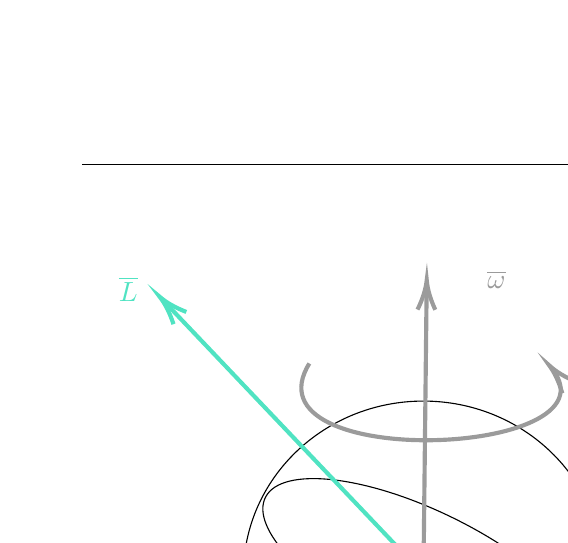
\begin{tikzpicture}[x=0.75pt,y=0.75pt,yscale=-1,xscale=1]
%uncomment if require: \path (0,280.4375); %set diagram left start at 0, and has height of 280.4375

%Shape: Ellipse [id:dp20504390100659775] 
\draw   (252.02,165.95) .. controls (252.02,119.84) and (290.85,82.46) .. (338.76,82.46) .. controls (386.66,82.46) and (425.5,119.84) .. (425.5,165.95) .. controls (425.5,212.06) and (386.66,249.44) .. (338.76,249.44) .. controls (290.85,249.44) and (252.02,212.06) .. (252.02,165.95) -- cycle ;
%Shape: Ellipse [id:dp5392542745699761] 
\draw   (262.73,128.65) .. controls (270.67,113.66) and (311.14,118.2) .. (353.13,138.8) .. controls (395.12,159.4) and (422.73,188.25) .. (414.79,203.25) .. controls (406.85,218.24) and (366.37,213.7) .. (324.38,193.1) .. controls (282.39,172.5) and (254.79,143.65) .. (262.73,128.65) -- cycle ;
%Straight Lines [id:da927531773364582] 
\draw [color={rgb, 255:red, 80; green, 227; blue, 194 }  ,draw opacity=1 ][line width=1.5]    (338.76,165.95) -- (213.71,34.34) ;
\draw [shift={(211.64,32.17)}, rotate = 406.46000000000004] [color={rgb, 255:red, 80; green, 227; blue, 194 }  ,draw opacity=1 ][line width=1.5]    (14.21,-4.28) .. controls (9.04,-1.82) and (4.3,-0.39) .. (0,0) .. controls (4.3,0.39) and (9.04,1.82) .. (14.21,4.28)   ;
%Curve Lines [id:da9106198351599886] 
\draw [color={rgb, 255:red, 155; green, 155; blue, 155 }  ,draw opacity=1 ][line width=1.5]    (283.79,64.34) .. controls (251.4,116.59) and (433.38,109.72) .. (401.01,67.27) ;
\draw [shift={(399.38,65.3)}, rotate = 408.15] [color={rgb, 255:red, 155; green, 155; blue, 155 }  ,draw opacity=1 ][line width=1.5]    (14.21,-4.28) .. controls (9.04,-1.82) and (4.3,-0.39) .. (0,0) .. controls (4.3,0.39) and (9.04,1.82) .. (14.21,4.28)   ;
%Straight Lines [id:da002180033456064989] 
\draw [color={rgb, 255:red, 155; green, 155; blue, 155 }  ,draw opacity=1 ][line width=1.5]    (338.76,165.95) -- (340.31,27.22) ;
\draw [shift={(340.34,24.22)}, rotate = 450.64] [color={rgb, 255:red, 155; green, 155; blue, 155 }  ,draw opacity=1 ][line width=1.5]    (14.21,-4.28) .. controls (9.04,-1.82) and (4.3,-0.39) .. (0,0) .. controls (4.3,0.39) and (9.04,1.82) .. (14.21,4.28)   ;


% Text Node
\draw (373.94,23.88) node  [color={rgb, 255:red, 155; green, 155; blue, 155 }  ,opacity=1 ]  {$\overline{\omega }$};
% Text Node
\draw (196.6,28.45) node  [color={rgb, 255:red, 80; green, 227; blue, 194 }  ,opacity=1 ]  {$\overline{L}$};


\end{tikzpicture}
\caption{Angular momentum vector from the moment of inertia tensor and angular velocity vector.}
\label{ang_mo_figure}
		\end{centering}
		\end{figure}

\begin{example} 
Consider the acquisition of the angular momentum vector via the action of the moment of inertia $\boldsymbol{tensor}$ on the angular velocity vector.
		
		\begin{equation}
		L_{i} = I_{ij}\omega^{j}
		\label{eq:angular_momentum}
		\end{equation}
		$I_{ij}$ : Moment of inertia tensor
	\end{example}
	Tensors are objects with multiple potential arguments on which they act linearly and can be characterized by different ranks or types. The ranks of each tensor correspond to the number of vector and or dual vector arguments the tensor will transform. For clarity, we will write tensors in the form of $\boldsymbol{T}(\_,\_,\_,\_)$ for now to help illustrate the tensor rank.
		\begin{example}
		$\boldsymbol{T}(\bar{V},\bar{W}) = C$ is a tensor of rank (0,2)\\
		$\boldsymbol{T}: T_{p} \times T_{p} \to \mathbb{R}$
		\end{example}
		
		\begin{example}
		$\boldsymbol{S}(\utilde{\omega},\bar{V}) = C$ is a tensor of rank (1,1)\\
		$\boldsymbol{S} : T^{*} _{p} \times T_{p} \to \mathbb{R}$
		\end{example}
		
		\begin{example}
		$\boldsymbol{R}(\utilde{\omega},\utilde{\alpha}) = C$ is a tensor of rank (2,0)\\
		$\boldsymbol{R} : T^{*} _{p} \times T^{*} _{p} \to \mathbb{R}$
		\end{example}
		
	A tensor of rank $(k,l)$ is a multilinear map of $k$ dual vectors and $l$ vectors to $\mathbb{R}$. In equation \eqref{eq:mapping}, $\times$ is a Cartesian product of the dual vector and vector spaces. As inferred from the last examples, a scalar is a type $(0,0)$ tensor, a dual vector is a type $(0,1)$ tensor and a vector is a type $(1,0)$ tensor.
	
		\begin{equation}
		\begin{aligned}
		\boldsymbol{T} : \underbrace{T^{*} _{p} \times ... \times T^{*} _{p}}_{k} \times \underbrace{T_{p} \times ... \times T_{p}}_{l} &\to \mathbb{R}
		\end{aligned}
		\label{eq:mapping}
		\end{equation}
	\begin{example}
	Tensor multilinearity can be seen in this tensor of type $(1,1)$.
	\begin{equation}
	\boldsymbol{T}(a\utilde{\alpha} + b\utilde{\beta}, c\bar{v} + d\bar{w}) = ac\boldsymbol{T}(\utilde{\alpha}, \bar{v}) + ad\boldsymbol{T}(\utilde{\alpha}, \bar{w}) + bc\boldsymbol{T}(\utilde{\beta}, \bar{v}) + bd\boldsymbol{T}(\utilde{\beta}, \bar{w})
	\end{equation}
	\end{example}
		Each rank $(k,l)$ tensor is a member of a vector space. Tensors of the same rank can be added, resulting in another tensor of that same rank. 
	
	\newpage
	
	\section{Tensor products}\label{sec:class_style}
	
    The tensor product operation $\otimes$ can be used to construct a basis for the space. Therefore, by taking the tensor product of a tensor $\boldsymbol{T}$ of rank $(k,l)$ and a tensor $\boldsymbol{S}$ of rank $(m,n)$, we define a new tensor $(\boldsymbol{T}$ $\otimes$ $\boldsymbol{S})$ of rank $(k+m, l+n)$.
	\begin{example}
	The tensor product between a vector and dual vector acting on a dual vector and vector argument results in a number.
	\begin{equation}
	( \bar{V} \otimes\utilde{\omega}) (\utilde{\alpha}, \bar{w}) = [\bar{V}(\utilde{\alpha})][\utilde{\omega}(\bar{w})]
	\label{eq:TP1}
	\end{equation}
	\end{example}
	
	 We can construct the basis that spans the vector space of the tensor by the tensor product of the dual vector and or vector bases.
	\begin{example}
	Basis of rank $(2,0)$ tensor : $\bar{e}_{(\mu)} \otimes \bar{e}_{(\nu)}$\\
	Basis of rank $(1,1)$ tensor : $\bar{e}_{(\mu)} \otimes \utilde{\theta}^{(\nu)}$\\
	Basis of rank $(0,2)$ tensor : $\utilde{\theta}^{(\mu)} \otimes \utilde{\theta}^{(\nu)}$
	\end{example}
	
	It can be seen that a tensor of rank $(2,0)$ contains 16 objects from the tensor product operation of the vector bases.
	\begin{equation}
	\begin{aligned}
	&\bar{e}_{(0)} \otimes \bar{e}_{(0)}\\
	&\bar{e}_{(0)} \otimes \bar{e}_{(1)} \\
	&. \\
	&. \\
	&. \\
	\boldsymbol{T} &= T^{\mu\nu} \bar{e}_{(\mu)} \otimes \bar{e}_{(\nu)}
	\label{eq:Tobjects}
	\end{aligned}
	\end{equation}
	
	The tensor products of the vector and dual vector bases corresponding to the tensor rank can be generalized:
	
	\begin{equation}
	(k,l) : \bar{e}_{(\mu_{1})} \otimes ... \otimes \bar{e}_{(\mu_{k})} \otimes \utilde{\theta}^{(\nu_{1})} \otimes ... \otimes \utilde{\theta}^{(\nu_{l})}
	\label{eq:Trank}
	\end{equation}
	We can extend this description of a rank $(k,l)$ tensor to any tensor.
	\begin{example}
	The metric tensor $\boldsymbol{g}$, a rank $(0,2)$ tensor is described as:
	\begin{equation}
	\boldsymbol{g} = g_{\mu\nu} \utilde{\theta}^{(\mu)} \otimes \utilde{\theta}^{(\nu)}
	\end{equation}
	\end{example}
	Thus, as seen in \eqref{eq:Tbasis}, a general tensor can be described as a long sum over $k$ vector components and $l$ dual vector components and the tensor products of the complete basis.
	\begin{equation}
	\boldsymbol{T} = \tensor{T}{^{\mu_{1}}^{\dots}^{\mu_{k}}_{\nu_{1}}_{\dots}_{\nu_{l}}} \bar{e}_{\mu_{(1)}} \otimes ... \otimes \utilde{\theta}^{\nu_{(l)}}
	\label{eq:Tbasis}
	\end{equation}
	
	We can now transition to writing tensors in the index notation, as demonstrated in the following example.
	\begin{example}
	For a rank $(2,0)$ tensor $\boldsymbol{S}$ : 
	\begin{equation}
	\begin{aligned}
	S(\utilde{\alpha},\utilde{\beta}) &= (S^{\mu\nu} \bar{e}_{(\mu)} \otimes \bar{e}_{(\nu)}) (\alpha_{\rho} \utilde{\theta}^{\rho}, \beta_{\sigma} \utilde{\theta}^{\sigma})\\
	&= S^{\mu\nu} \alpha_{\rho} \beta_{\sigma} (\bar{e}_{(\mu)} \otimes \bar{e}_{(\nu)}) (\utilde{\theta}^{(\rho)}, \utilde{\theta}^{(\sigma)})\\
	\end{aligned}
	\label{eq:index_ex1}
	\end{equation}
	Recall the rule: \\
	\begin{equation}
	\begin{aligned}
	\bar{e}_{(\mu)} (\utilde{\theta}^{(\rho)}) &= \utilde{\theta}^{(\rho)} (\bar{e}_{(\mu)})\\
	&= \tensor{\delta}{^\rho_\mu}
	\end{aligned}
	\label{eq:kronecker}
	\end{equation}
	Equation \eqref{eq:index_ex1} continues as thus:
	\begin{equation}
	S^{\mu\nu} \alpha_{\rho} \beta_{\sigma} \tensor{\delta}{^\rho_\mu} \tensor{\delta}{^\sigma_\nu}\\
	= S^{\mu\nu} \alpha_{\mu} \beta_{\nu}
	\label{eq:index_ex2}
	\end{equation}
	The tensor $\boldsymbol{S}$ acts upon two dual vectors and returns a scalar.
	\end{example}
	
	
	\newpage
	
	\section{Lorentz transformations}\label{sec:lorentz}
	Now, we can apply the Lorentz transformation with our current knowledge of transforming vectors and dual vectors. Notice in the following example that the Lorentz transformation transforms between frames of the tensor components and the bases, but leaves the tensor itself invariant.
	\begin{example}
	For a $(1,1)$ tensor, the Lorentz transformation acting on the components can be described as:
	\begin{equation}
	\begin{aligned}
	\boldsymbol{T} &= \tensor{T}{^\mu_\nu} \bar{e}_{(\mu)} \otimes \utilde{\theta}^{(\nu)}\\
	&= \tensor{T}{^{\mu'}_{\nu'}} \bar{e}_{(\mu')} \otimes \utilde{\theta}^{(\nu')}\\
	\label{eq:lorentz1}
	\end{aligned}
	\end{equation}
	Recall:\\
	\begin{equation}
	\bar{e}_{(\mu')} = \tensor{\Lambda}{^\nu_{\mu'}} \bar{e}_{(\nu)}
	\label{eq:lorentz2}
	\end{equation}
	
	For a $(2,1)$ tensor, the Lorentz transformation is described as:
	\begin{equation}
	\boldsymbol{S} : \tensor{S}{^{\mu'}^{\nu'}_{\rho'}} = \tensor{\Lambda}{^{\mu'}_{\alpha}} \tensor{\Lambda}{^{\nu'}_{\beta}} \tensor{\Lambda}{^{\nu}_{\rho'}} \tensor{S}{^{\alpha}^{\beta}_{\nu}}
	\label{eq:lorentz3}
	\end{equation}
	\end{example}
	
	
\end{document}
